\documentclass{article}
\usepackage[utf8]{inputenc}
\usepackage{indentfirst}
\usepackage{listings}
\usepackage{xcolor}
\usepackage{graphicx}

\definecolor{mGreen}{rgb}{0,0.6,0}
\definecolor{mGray}{rgb}{0.5,0.5,0.5}
\definecolor{mPurple}{rgb}{0.58,0,0.82}
\definecolor{backgroundColour}{rgb}{0.95,0.95, 1}

\lstdefinestyle{CStyle}{
    backgroundcolor=\color{backgroundColour},   
    commentstyle=\color{mGreen},
    keywordstyle=\color{magenta},
    numberstyle=\tiny\color{mGray},
    stringstyle=\color{mPurple},
    basicstyle=\ttfamily\footnotesize,
    breakatwhitespace=false,         
    breaklines=true,                 
    captionpos=b,                    
    keepspaces=true,                 
    numbers=left,                    
    numbersep=5pt,                  
    showspaces=false,                
    showstringspaces=false,
    showtabs=false,                  
    tabsize=2,
    language=C
}

\title{CSE344 \protect\\ Systems Programming Course \protect\\ Final Project Report}
\author{Furkan Özev \protect\\161044036 }
\date{June $28^{th}$, 2020}

\begin{document}

\maketitle

\section{Main Idea}
\noindent In this project, there are 2 programs. A threaded server and a client. The server will load a graph from a text file, and use a dynamic pool of threads to handle incoming connections. The clients will connect to the server and request a path between two arbitrary nodes, and the server will provide this service.
\newline \newline Also server process will be a daemon. So, It should not possible to start 2 instances of the server process. Server process has no controlling terminal. And its inherited open files will close.
\newline \newline After the server process loads the graph from the input file into memory,The server process will communicate with the client processes through stream/TCP socket based connections. The server will possess a pool of POSIX threads, and in the form of an endless loop, as soon as a new connection arrives, it will forward that new connection to an available thread of the pool, and immediately continue waiting for a new connection. If no thread is available, then it will wait in a blocked status until a thread becomes available. The pool of threads will be created and initialized at the daemon’s startup, and each thread will execute in an endless loop, first waiting for a connection to be handed to them by the server, then handling it, and then waiting again, and so on.
\newline \newline Once a connection is established, the client will simply send two indexes i1 and i2, as two non negative integers, representing each one of the nodes of the graph, to the server, and wait for the server to reply with the path from i1 to i2. If the requested path from i1 to i2 has been already calculated during a past request, the thread handling this request should first check a cache, containing past calculations, and if the requested path is present in it, the thread should simply use it to respond to the client, instead of recalculating it. Otherwise, it will use breadth-first search to find a path from i1 to i2. If it is not present in the cache then it must inevitably calculate it with breadth-first search, respond to the client, and add the newly calculated path into the data structure, so as to accelerate future requests. If no path is possible between the requested nodes, then the server will respond accordingly.
\newline \newline The cache will be common to all threads of the pool and can be thought of as a “database”. It must not contain duplicate entries, and it must support fast access/search. This database includes multiple and serious synchronization. It used readers/writers paradigm, by prioritizing writers to provide synchronization. Readers are the threads attempting to search the data structure to find out whether a certain path is in it or not. Writers are the threads that have calculated a certain path and now want to add it into the data structure.
\newline \newline If the server receives the SIGINT signal it will wait for its ongoing threads to complete, return all allocated resources, and then shutdown gracefully.
\newline \newline Thread pool would be “dynamic”. This means it will not have a fixed number of threads, instead the number of threads will increase depending on how busy the server is. Specifically, every time that the load of the server reaches 75\%, i.e. 75\% of the threads become busy,  then the pool size will be enlarged by 25\%.
\newline \newline The client is simple. Given the server’s address and port number, it will simply request a path from node i1 to i2 and wait for a response, while printing its output on the terminal.

\section{Server Code Flow}
\subsection{Main Thread Flow}
\noindent To measures against double instantiation,  When the program starts, it creates a temporary file. If a second server tries to open this file, it will get an error. Thus, double instantiation will be prevented.

\begin{lstlisting}[style=CStyle]
...

int fd = open("/tmp/daemonLock", O_CREAT | O_EXCL);
if(fd == -1)
{
  fprintf(stderr, "\nIt should not be possible to start 2 instances of the server process\n\n");
  exit(EXIT_FAILURE);
}
\end{lstlisting}

\noindent After the parameters are read, the values are checked.Number of port mustn't be negative, number of threads can be at least 2, number of threads must not bigger than maximum allowed number of threads.
\begin{lstlisting}[style=CStyle]
  ...

if(port < 0)
{
  fprintf(stderr, "-p(number of port) mustn't be negative.\n");
  unlink("/tmp/daemonLock");
  exit(EXIT_FAILURE);
}

if(threadNumber < 2)
{
  fprintf(stderr, "-s(number of threads) can be at least 2.\n");
  unlink("/tmp/daemonLock");
  exit(EXIT_FAILURE);
}

if(threadNumber > maxThread)
{
  fprintf(stderr, "-s(number of threads) must not bigger than -x(maximum allowed number of threads)\n");
  unlink("/tmp/daemonLock");
  exit(EXIT_FAILURE);
}
  
  ...
    
\end{lstlisting}

\noindent The becomeDaemon() function is called. Thus, process's terminal connection is canceled and inherited open files are closed. Then the input files are opened and the hands of the SIGINT signal are changed.
\begin{lstlisting}[style=CStyle]
 ...

becomeDaemon();
fd1 = fopen(filePath, "r");
fd2 = fopen(logPath, "w+");
signal(SIGINT, sigHandler);

 ...
\end{lstlisting}

\subsubsection{becomeDaemon}
\noindent It was made by looking at the 770 th page of the book.  Server process has no controlling terminal.  And its inherited open files will close
\begin{lstlisting}[style=CStyle]

...
switch(fork())
{
  case -1:
    return -1;
  case 0:
    break;
  default:
    exit(EXIT_SUCCESS);
}

if(setsid() == -1)
  return -1;

switch(fork())
{
  case -1:
    return -1;
  case 0:
    break;
  default:
    exit(EXIT_SUCCESS);
}

umask(0);

maxfd = sysconf(_SC_OPEN_MAX);
if(maxfd == -1)
  maxfd = 8192;

// Close all of its inherited open files
for(fd = 0; fd < maxfd; fd++)
  close(fd);
    
...
\end{lstlisting}

\noindent It will initialize graph. The server process will load the graph to memory from its input file. Then, it will initialize catch. Then pool threads and dynamic coordinate thread are created.
\begin{lstlisting}[style=CStyle]
...
initGraph(&graph1);
loadGraph(&graph1, fd1);
initCatch(&catch1, graph1.a, graph1.b, graph1.c);

// Create pool threads. Thread take number.
for(i = 0; i < threadNumber; i++)
    pthread_create(&(thread_id[i]), NULL, &thread_function, indexThread[i]);
    
// Create dynamic coordinate thread
pthread_create(&thread_pool, NULL, &thread_coord_pool, NULL);

...
\end{lstlisting}

\noindent Necessary socket operations are made to communicate between the server and clients.
\begin{lstlisting}[style=CStyle]
...
struct sockaddr_in serverAddr;
int socket2;
int addrlen = sizeof(serverAddr);
int opt1 = 1;

// Create socket file descriptor 
socket1 = socket(AF_INET, SOCK_STREAM, 0);

// Forcefully attaching socket to the port
setsockopt(socket1, SOL_SOCKET, SO_REUSEADDR | SO_REUSEPORT, &opt1, sizeof(opt1));

serverAddr.sin_family = AF_INET;; 
serverAddr.sin_addr.s_addr = INADDR_ANY; 
serverAddr.sin_port = htons(port);

// Binds the socket to the address and port number
bind(socket1, (struct sockaddr *)&serverAddr, sizeof(serverAddr))

//  It waits for the client to approach the server to make a connection
listen(socket1, 4096)
...
\end{lstlisting}
\noindent Main Thread: Endless loop, it just check sigint signal arrives. First it accept a connection. Then check system load capacity. If it has reached, it waits for the pool coordinate thread to create new threads. If it reaches the maximum number of threads, the threads are expected to finish. Then it give socket to any thread. Any thread is expected to receive the sent socket. The same process repeats. Mutexes are used in this section as there are critical regions.
\begin{lstlisting}[style=CStyle]
...
while(flagint == 0)
{
    socket2 = accept(socket1, (struct sockaddr *)&serverAddr, (socklen_t*)&addrlen);
    // Lock pool coordinate thread
    pthread_mutex_lock(&mutex3);
    // Lock pool threads
  pthread_mutex_lock(&mutex1);
  
  // Connection counter increased by 1
  pcount2 += 1;
  
  // Checks whether the capacity has reached 75%.
  // If it has reached, it waits for the pool coordinate thread to create new threads.
  while(capacity >= 75 && threadNumber != maxThread)
  {
      pthread_cond_broadcast(&pempty);
    pthread_cond_wait(&pfull, &mutex3);
  }
  pthread_cond_broadcast(&pempty);
  pthread_mutex_unlock(&mutex3);
  
  // If it reaches the maximum number of threads, the threads are expected to finish.
  while(pcount2 > maxThread || pcount3 >= threadNumber))
      pthread_cond_wait(&cempty, &mutex1);
      
  // Enqueue the provided socket to queue, And increase counters
  enqueue(&ports, socket2);
  pcount += 1;
  pcount3 += 1;

  pthread_cond_broadcast(&cfull);
  pthread_mutex_unlock(&mutex1);
  
  // It is ensured that the connection provided by the main thread is forwarded to any thread.
  pthread_mutex_lock(&tmutex);
  while(tcount == 1)
    pthread_cond_wait(&tempty, &tmutex);
  tcount = 1;
  pthread_cond_broadcast(&tfull);
  pthread_mutex_unlock(&tmutex);
}
...
\end{lstlisting}
\noindent After sigint signal, it will join threads, close socket, close files, unlink daemon file, free all allocated memory.
\begin{lstlisting}[style=CStyle]
...
// Join threads
for(i = 0; i < threadNumber; i++)
    pthread_join(thread_id[i], NULL);
    
pthread_join(thread_pool, NULL);

// Close files and sockets
close(socket1);
fclose(fd1);
fclose(fd2);
close(fd);

// Deallocate all memory
freeAll();

// unlink temprory file
unlink("/tmp/daemonLock");
...
\end{lstlisting}
\subsection{Pool Threads Flow}
\noindent Endless loop, it just check sigint signal arrives. It expects a connection to be provided by the main thread. When the main thread provides connection, any thread wakes up. It takes the socket and thus gets the nodes from the client. The message type of the client is "node1-node2". Parse this message. It informs the main thread that it has received the connection.
\begin{lstlisting}[style=CStyle]
...
claf = 0;
while(flagint == 0)
{
  pthread_mutex_lock(&mutex1);
  // If any thread completes an loop
  if(cflag == 1)
  {
    // Decrase counters
    pcount3 -= 1;
    pcount2 -= 1;
    pthread_cond_signal(&cempty);
  }
  else
    cflag = 1;
  // Waits to be awakened by the main thread.
  while(flagint == 0 && pcount == 0)
    pthread_cond_wait(&cfull, &mutex1);
  
  // Take socket from queue
  temp = dequeue(&ports);
  pcount -= 1;
  
  // Indicates that the connection was received by any thread.
  pthread_mutex_lock(&tmutex);
  while(flagint == 0 && tcount == 0)
    pthread_cond_wait(&tfull, &tmutex);
  tcount = 0;
  pthread_cond_broadcast(&tempty);
  pthread_mutex_unlock(&tmutex);

  pthread_cond_broadcast(&cempty);
  pthread_mutex_unlock(&mutex1);

  // Parse message, then get nodes.
  for(i = 0; buffer[i] != '-'; i++);
  strncpy(buffer4, buffer, i);
  buffer4[i] = '\0';
  node1 = atoi(buffer4);
  strncpy(buffer4, &(buffer[i+1]), strlen(buffer)-i);
  buffer4[strlen(buffer)-i] = '\0';
  node2 = atoi(buffer4);
...
\end{lstlisting}
\noindent In cache access, the reader-writer paradigm is used. Reader paradigm: First search in cache, if path does not exist in cache, it will breadth-first search in graph. Writer paradigm: If it finds path with bfs, it will send path to client and write this path to cache. If path exists in cache, it will send path to client. If path is not found, it reports this to the client.
\begin{lstlisting}[style=CStyle]
...
/ Readers are the threads attempting to search the data structure to find out whether a certain path is in it or not
pthread_mutex_lock(&mutex2);
while((AW + WW) > 0)
{
  WR++;
  pthread_cond_wait(&okToRead, &mutex2);
  WR--;
}
AR++;
pthread_mutex_unlock(&mutex2);

sprintf(logbuf, "Thread #%d: searching database for a path from node %d to node %d", x, node1, node2);
printLog(logbuf);

res = 0;
// Determine indexs, It is checked whether the path is in catch or not.
if(node1 >= catch1.sizea || node2 >= catch1.sizeb)
  index = -2;
else
{
  index = -1;
  nodetemp = catch1.index[node1]->front;
  while(nodetemp != NULL)
  {
    if(nodetemp->item == node2)
    {
      index = nodetemp->index;
      break;
    }
    nodetemp = nodetemp->next;
  }
}

// If index is negative, path does not exist in cache
// If not, it is the index where the path is located.
if(index != -1 && index != -2)
{
  // Converts path to string
  strcpy(buffer2, " ");
  strcpy(buffer3, " ");
  nodetemp = catch1.paths[index]->front;
  i = 0;
  while(nodetemp != NULL)
  {
    sprintf(buffer3, "%d", nodetemp->item);
    if(i == 0)
      strcpy(buffer2, buffer3);
    else if(nodetemp->next != NULL)
    {
      strcat(buffer2, "->");
      strcat(buffer2, buffer3);
    }
    else
    {
      strcat(buffer2, "->");
      strcat(buffer2, buffer3);
    }

    nodetemp = nodetemp->next;
    i += 1;
  }

  // The path is sent to the client.
  pthread_mutex_lock(&sendmutex);
  sprintf(logbuf, "Thread #%d: path found in database: %s", x, buffer2);
  printLog(logbuf);
  send(temp, buffer2, strlen(buffer2), 0);
  close(temp);
  pthread_mutex_unlock(&sendmutex);
}
else
{
  sprintf(logbuf, "Thread #%d: no path in database, calculating %d->%d ", x, node1, node2);
  printLog(logbuf);
}

// Reading process completed.
// It awakens the waiting threads.
pthread_mutex_lock(&mutex2);
AR--;
if(AR == 0 && WW > 0)
  pthread_cond_signal(&okToWrite);
pthread_mutex_unlock(&mutex2);

// Search path with bfs algroithm
if(index == -1)
{
  // If bfs return -1, there is no path
  // If not, there is a path and it will fill resArr array
  res = bfs(&graph1, node1, node2, resArr);

  // Writers are the threads that have calculated a certain path and now want to add it into the data structure
  pthread_mutex_lock(&mutex2);
  while((AW + AR) > 0)
  {
    WW++;
    pthread_cond_wait(&okToWrite, &mutex2);
    WW--;
  }
  AW++;
  pthread_mutex_unlock(&mutex2);

  if(res != -1)
  {
    // Converts path to string
    strcpy(buffer2, " ");
    strcpy(buffer3, " ");
    for(i = 0; i <= res; i++)
    {
      sprintf(buffer3, "%d", resArr[i]);
      if(i == 0)
        strcpy(buffer2, buffer3);
      else if(i != res)
      {
        strcat(buffer2, "->");
        strcat(buffer2, buffer3);
      }
      else
      {
        strcat(buffer2, "->");
        strcat(buffer2, buffer3);
      }
    }

    // The path is sent to the client.
    pthread_mutex_lock(&sendmutex);
    sprintf(logbuf, "Thread #%d: path calculated: %s", x, buffer2);
    printLog(logbuf);
    send(temp, buffer2, strlen(buffer2), 0);
    close(temp);
    pthread_mutex_unlock(&sendmutex);

    // Path found in BFS is added to cache
    enqueue2(catch1.index[node1], node2, catch1.count);
    catch1.count += 1;
    if(catch1.count == 1)
      catch1.paths = (Queue**) calloc(catch1.count, sizeof(Queue*));
    else
      catch1.paths = (Queue**) realloc(catch1.paths, catch1.count * sizeof(Queue*));

    catch1.paths[catch1.count - 1] = (Queue*) malloc(sizeof(Queue));
    catch1.paths[catch1.count - 1]->front = NULL;
    catch1.paths[catch1.count - 1]->rear = NULL;

    for(i = 0; i <= res; i++)
      enqueue(catch1.paths[catch1.count - 1], resArr[i]);
  }

  // Writting process completed.
  // It awakens the waiting threads.
  pthread_mutex_lock(&mutex2);
  AW--;
  if(WW > 0)
    pthread_cond_signal(&okToWrite);
  else if (WR > 0)
    pthread_cond_broadcast(&okToRead);
  pthread_mutex_unlock(&mutex2);
}

// Path not found with bfs or in cache
if(res == -1 || index == -2)
{
  pthread_mutex_lock(&sendmutex);
  sprintf(logbuf, "Thread #%d: path not possible from node %d to %d ", x, node1, node2);
  printLog(logbuf);
  send(temp, "N", 1, 0);
  close(temp);
  pthread_mutex_unlock(&sendmutex);
}
  
...
\end{lstlisting}

\subsection{Pool Coordinate Thread Flow}
\noindent This thread coordinate thread pool. When systeam load is reached 75\%, it will expand pool with creating new threads.
\noindent Checks whether the capacity has reached 75\%. If it has reached, it will start for the extend pool, If not, it will wait.
\newline \noindent The pool size will be enlarged by 25\%, so it will calculate new size.
\newline \noindent If 25\% excess of the current thread is still equal to it and 1 excess is possible, 1 is increased.
\newline \noindent If 25\% excess of the current thread is not equal to it and pool will enlarged with new thread number.
\newline \noindent Otherwise, Thread has reached the maximum number.
\newline \noindent It will create new thread for enlarge pool and it will print new system load and thread number in pool 

\begin{lstlisting}[style=CStyle]
...
//Endless loop, it just check sigint signal arrives.
while(flagint == 0)
{
    // Critical section between this thread and main thread
  pthread_mutex_lock(&mutex3);
  while(flagint == 0 && capacity < 75 && threadNumber != maxThread)
    pthread_cond_wait(&pempty, &mutex3);
  if(flagint != 0)
  {
    pthread_cond_broadcast(&pfull);
    pthread_mutex_unlock(&mutex3);
    break;
  }

  temp2 = threadNumber;
  capacity = ((double)pcount2) / ((double)threadNumber) * 100;

  // the pool size will be enlarged by 25%
  temp = threadNumber;
  newamount = round(threadNumber * 1.25);

  // If 25% excess of the current thread is still equal to it and 1 excess is possible, 1 is increased.
  if(threadNumber == newamount && (newamount + 1) <= maxThread)
    threadNumber = newamount + 1;
  // If 25% excess of the current thread is not equal to it and pool will enlarged with new thread number.
  else if(threadNumber != newamount && newamount <= maxThread)
    threadNumber = newamount;
  // Otherwise, Thread has reached the maximum number.
  else
    threadNumber = maxThread;

  // Create new thread for enlarge pool.
  if(temp != threadNumber)
  {
    thread_id = (pthread_t*) realloc(thread_id, threadNumber * sizeof(pthread_t));
    indexThread = (int**) realloc(indexThread, threadNumber * sizeof(int*));

    for( ; temp < threadNumber; temp++)
    {
      indexThread[temp] = malloc(sizeof(int));
      *(indexThread[temp]) = temp;
      if(pthread_create(&(thread_id[temp]), NULL, &thread_function, indexThread[temp]) != 0)
      {
        sprintf(logbuf, "errno = %d: %s pthread_create\n", errno, strerror(errno));
        printLog(logbuf);
        unlink("/tmp/daemonLock");
        exit(EXIT_FAILURE);
      }
    }
  }

  // Print new system load and thread number in pool
  if(temp2 != threadNumber)
  {
    sprintf(logbuf, "System load %lf%%, pool extended to %d threads", capacity, threadNumber);
    printLog(logbuf);
  }

  pthread_cond_broadcast(&pfull);
  pthread_mutex_unlock(&mutex3);
}
return NULL;
...
\end{lstlisting}

\subsection{Graph}
\noindent For graph, Adjacency list (queue) is kept in queue structure. The Load function also keeps the maximum number of nodes while reading the file. Therefore, these numbers are given to the graph at the beginning. When creating the Graph list, it determines its size based on this number amounts. This saves memory as much as possible.

\begin{lstlisting}[style=CStyle]
graph->size = graph->a;
graph->adjList = (Queue**) calloc(graph->size, sizeof(Queue*));
for(i = 0; i < graph->size; i++)
{
  graph->adjList[i] = (Queue*) malloc(sizeof(Queue));
  graph->adjList[i]->front = NULL;
  graph->adjList[i]->rear = NULL;
}
graph->nodelist = (int *) calloc(graph->b, sizeof(int));
\end{lstlisting}

\noindent Then, the elements are added to the graph in order. While doing this, it checks whether the edge has been added before.
\begin{lstlisting}[style=CStyle]
void addEdge(Graph* graph, int x, int y)
{
  if(existInList(graph->adjList[x], y) == -1)
  {
    enqueue(graph->adjList[x], y);
    graph->edges += 1;
  }

  graph->nodelist[x] = 1;
  graph->nodelist[y] = 1;
}
\end{lstlisting}

\subsection{Cache}
\noindent The Load function also keeps the maximum number of nodes while reading the file. Therefore, these numbers are given to the cache at the beginning. When creating the cache list, it determines its size based on this number amounts. This saves memory as much as possible.
\begin{lstlisting}[style=CStyle]
void initCatch(Catch* catch, int a, int b, int c)
{
  int i;
  catch->sizea = a;
  catch->sizeb = b;
  catch->sizec = c;
  catch->count = 0;

  catch1.index = (Queue**) calloc(catch->sizea, sizeof(Queue*));
  for(i = 0; i < catch->sizea; i++)
  {
    catch->index[i] = (Queue*) malloc(sizeof(Queue));
    catch->index[i]->front = NULL;
    catch->index[i]->rear = NULL;
  }
  catch->paths = NULL;
}
\end{lstlisting}
\noindent The previously calculated paths are kept in cache. Paths are kept in a queue. The indexes of the paths are kept in another 2-dimensional queue. When a path is queried, first the index is found from the 2D queue and then the pathe is accessed directly.

\begin{lstlisting}[style=CStyle]
// Search index in 2D queue
// For example 25->150
// node1 = 25, node2 = 150
index = -1;
nodetemp = catch1.index[node1]->front;
while(nodetemp != NULL)
{
  if(nodetemp->item == node2)
  {
    index = nodetemp->index;
    break;
  }
  nodetemp = nodetemp->next;
}

// If index is negative, path does not exist in cache
// If not, it is the index where the path is located.
if(index != -1)
{
    // Paths in nodetemp. So it can be directly accessed.
    nodetemp = catch1.paths[index]->front;
}

\end{lstlisting}

\subsection{Signal Handler and Exit}

\noindent Replaces the value of the global variable (flagint) with 1. Therefore, the threads will understand that a sigint signal has arrived and will end after it have finished it job. It must wait for its ongoing threads to complete. So it will wakeup ongoing threads. Thus deadlock is prevented.
\begin{lstlisting}[style=CStyle]
if(sig == SIGINT)
{
  sprintf(logbuf, "Termination signal received, waiting for ongoing threads to complete.");
  printLog(logbuf);
  // Replaces the value of the global variable with 1.
  flagint = 1;
  if(socket1 != -1)
  {
    shutdown(socket1, SHUT_RD);
    close(socket1);
  }
  socket1 = -2;

  // It will wait for its ongoing threads to complete. So it will wakeup ongoing threads.
  pthread_cond_broadcast(&cfull);
  pthread_cond_broadcast(&pfull);
  pthread_cond_broadcast(&tfull);
    pthread_cond_broadcast(&cempty);
  pthread_cond_broadcast(&pempty);
  pthread_cond_broadcast(&tempty);
}
\end{lstlisting}

\subsection{Logging}

\noindent Threads directly call this function for printing. To prevent conflict in the file, it is locked before printing, after the process is completed, mutex unlock is done. Thus, 1 printing will be done at the same time. Necessary actions are taken for timestamp. The message is printed on the file.
\begin{lstlisting}[style=CStyle]
void printLog(char* str)
{
  pthread_mutex_lock(&printmutex);
  time_t ltime;
  struct tm lresult;
  char stime[32];
  size_t n;

  ltime = time(NULL);
  localtime_r(&ltime, &lresult);
  asctime_r(&lresult, stime);
  n = strlen(stime);
  if(n && stime[n-1] == '\n') stime[n-1] = '\0';
  fprintf(fd2, "[%s] %s\n", stime, str);
  pthread_mutex_unlock(&printmutex);
}

\* Like that:
[Sun Jun 28 15:28:37 2020] Executing with parameters:
[Sun Jun 28 15:28:37 2020] -i p2p-Gnutella08.txt
[Sun Jun 28 15:28:37 2020] -p 45
*/
\end{lstlisting}

\section{Client Code Flow}
\noindent After the parameters are read, the values are checked.Number of port mustn't be negative, node1 and node2 mustn't negative.
\begin{lstlisting}[style=CStyle]
  ...

// Check values
if(port < 0)
{
  printf("-p(number of port) must be positive.\n");
  exit(EXIT_FAILURE);
}

if(node1 < 0)
{
  printf("-s(source node of the requested path) must not negative.\n");
  exit(EXIT_FAILURE);
}
if(node2 < 0)
{
  printf("-d(destination node of the requested path) must not negative.\n");
  exit(EXIT_FAILURE);
}
  
  ...
    
\end{lstlisting}
\noindent Necessary socket operations are made to communicate between the server and clients.
\begin{lstlisting}[style=CStyle]
...
// Create socket file descriptor 
if((socket1 = socket(AF_INET, SOCK_STREAM, 0)) < 0) 
{
  fprintf(stderr, "\nerrno = %d: %s Socket creation error\n\n", errno, strerror(errno));
  exit(EXIT_FAILURE);
}

serverAddr.sin_family = AF_INET; 
serverAddr.sin_port = htons(port);

// Convert IPv4 and IPv6 addresses from text to binary form
if(inet_pton(AF_INET, ip, &serverAddr.sin_addr)<=0)  
{
  fprintf(stderr, "\nerrno = %d: %s Invalid address/ Address not supported\n\n", errno, strerror(errno));
  exit(EXIT_FAILURE);
}

if(connect(socket1, (struct sockaddr *)&serverAddr, sizeof(serverAddr)) < 0) 
{
  fprintf(stderr, "\nerrno = %d: %s Connection Failed \n\n", errno, strerror(errno));
  exit(EXIT_FAILURE);
}

printf("Client (%d) connected and requesting a path from node %d to %d\n", pid, node1, node2);
// Send nodes to server
send(socket1, bufwrite, strlen(bufwrite), 0);

// Calculate response time
gettimeofday(&start, NULL);
// Take result from server
size = read(socket1, bufread, SIZE);
gettimeofday(&end, NULL);
long seconds = (end.tv_sec - start.tv_sec);
long micros = ((seconds * 1000000) + end.tv_usec) - (start.tv_usec);
double diff_t = (double) micros / 1000000;

// Server response
if(bufread[0] == 'N' || size == 0)
  printf("Server's response to (%d) : NO PATH, arrived in %lfseconds, shutting down\n", pid, diff_t);
else
  printf("Server's response to (%d) : %s, arrived in %lfseconds.\n", pid, bufread, diff_t);

close(socket1);
...
\end{lstlisting}

\section{Compile \& Run}
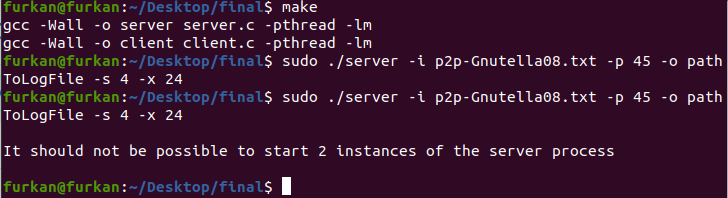
\includegraphics[width=\textwidth]{1.png} \newline
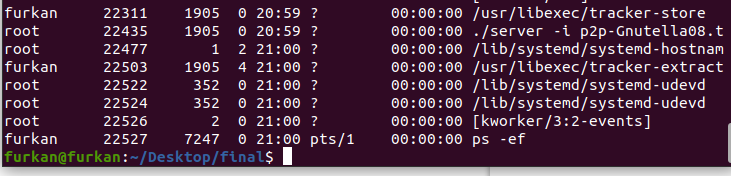
\includegraphics[width=\textwidth]{2.png} \newline
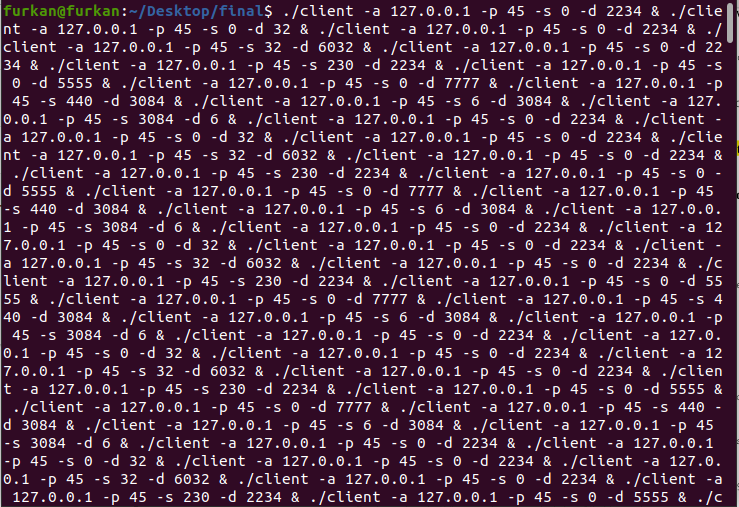
\includegraphics[width=\textwidth]{3.png} \newline
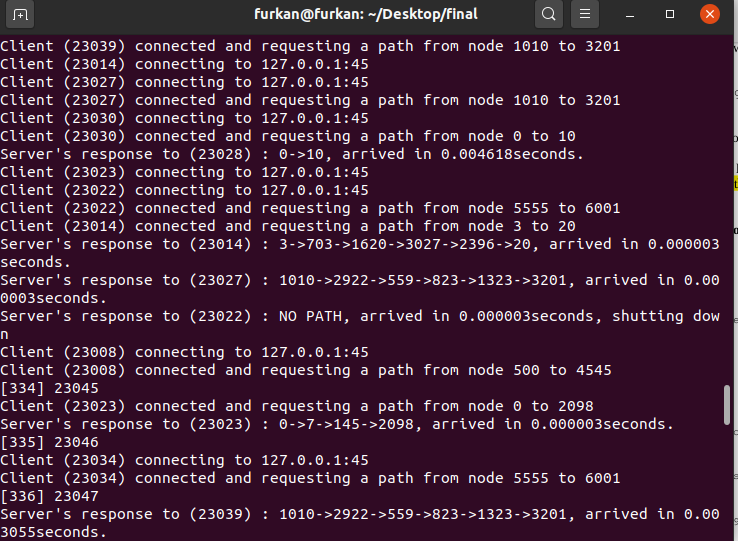
\includegraphics[width=\textwidth]{4.png} \newline
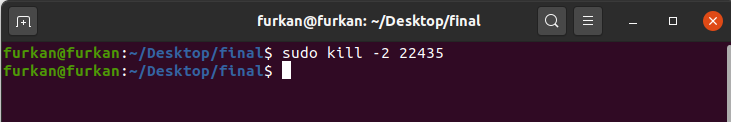
\includegraphics[width=\textwidth]{5.png} \newline
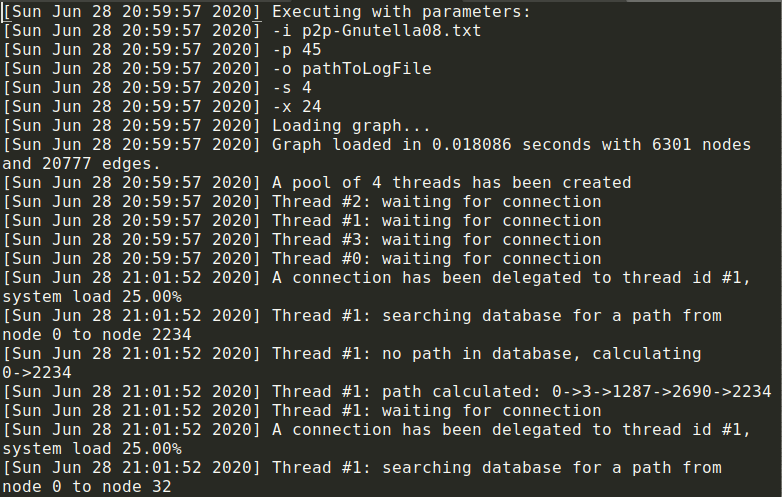
\includegraphics[width=\textwidth]{6.png} \newline
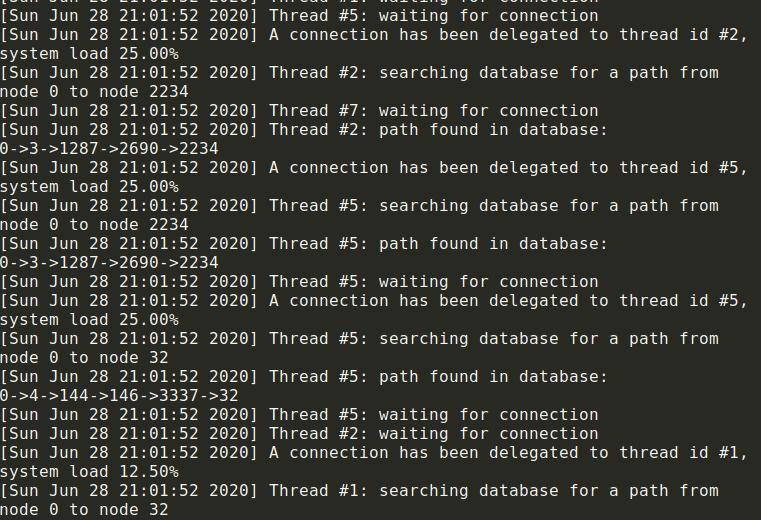
\includegraphics[width=\textwidth]{7.png} \newline
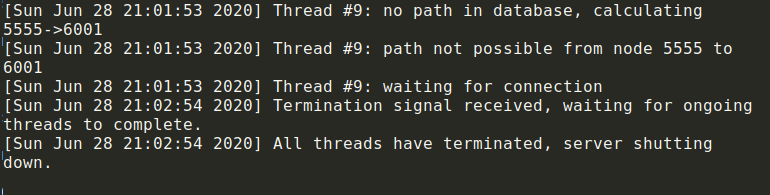
\includegraphics[width=\textwidth]{8.png} \newline

\section{Valgrind}

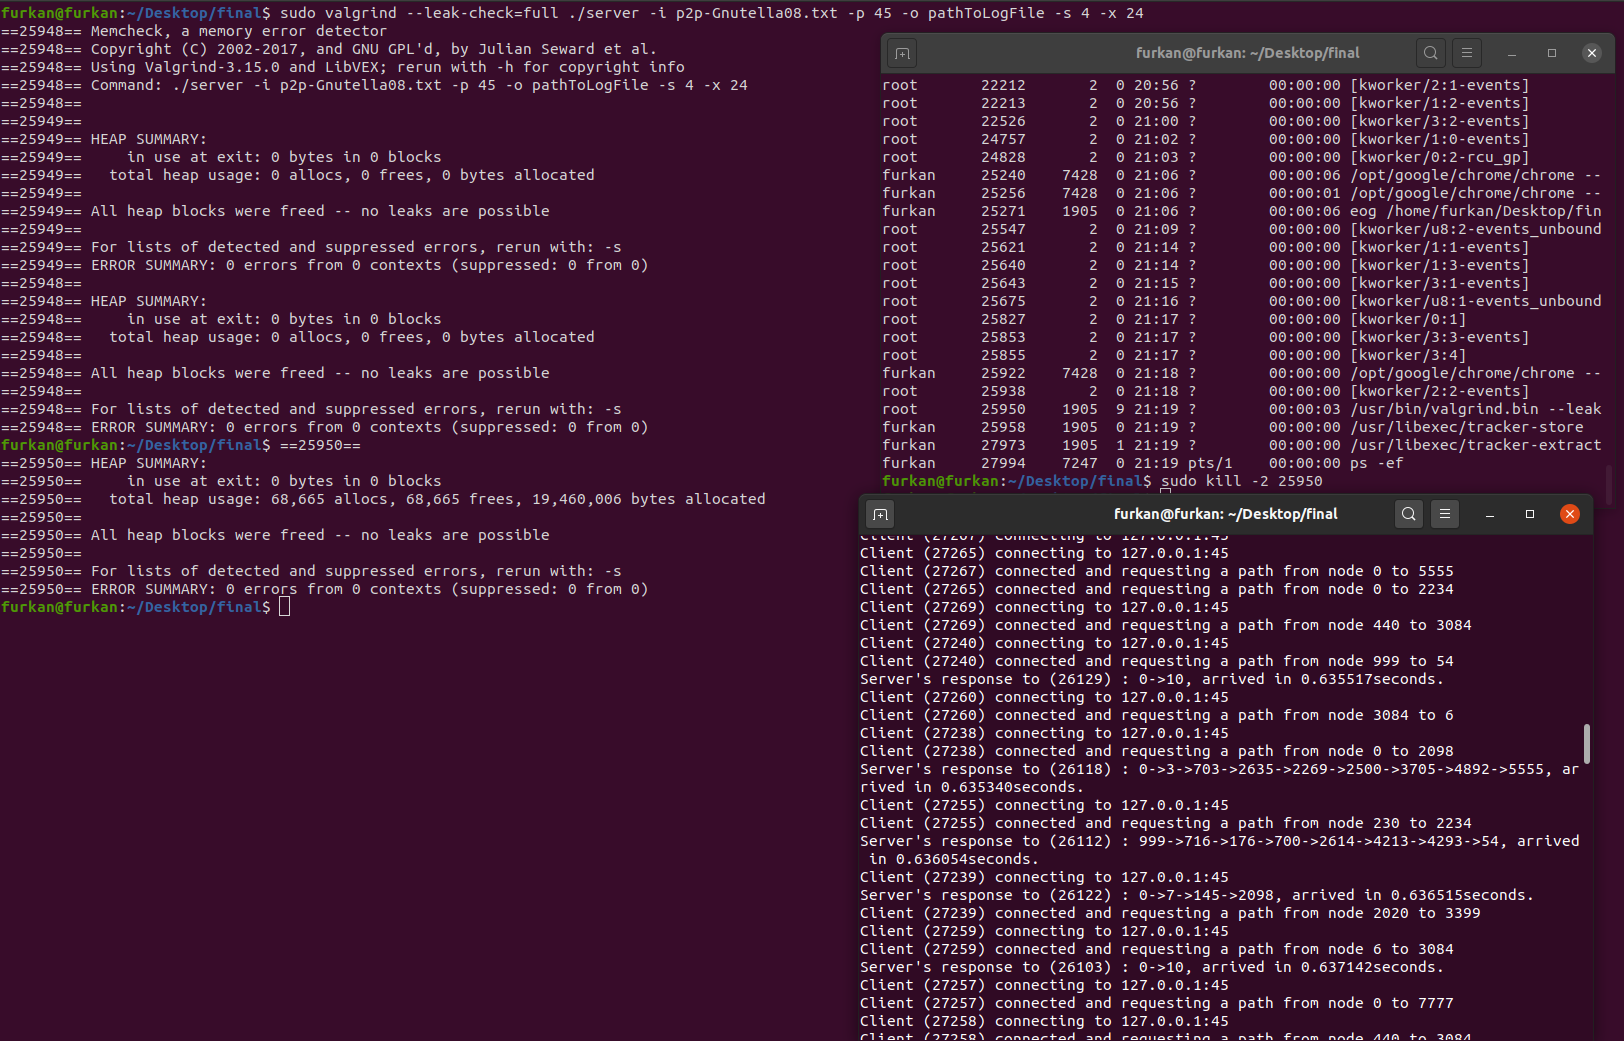
\includegraphics[width=\textwidth]{10.png} \newline

\end{document}